\documentclass[../main.tex]{subfiles}
% \documentclass[12pt, preprint,letterpaper]{article}
\usepackage[utf8]{inputenc}
\usepackage[english]{babel}
\usepackage{xspace} % For spacing
\usepackage{natbib} % For bib files
\usepackage{amsmath} % boldsymbol{} needs this.
\usepackage{mathrsfs} % For refrencing math environment
\usepackage[usenames,dvipsnames,svgnames,table]{xcolor} % For colors
\usepackage{etoolbox} % To compile in Atom
\usepackage{graphicx} % For figures
\graphicspath{{images/}{../images/}}
% \graphicspath{ {figures/} } % Put figures inside this directory and use pdf
\usepackage[parfill]{parskip} % to avoid indentation in paragraphs
\usepackage{enumitem} % for listing
\usepackage[ampersand]{easylist}
\ListProperties(Hide=100, Hang=true, Progressive=3ex, Style*=-- ,
Style2*=$\bullet$ ,Style3*=$\circ$ ,Style4*=\tiny$\blacksquare$ )    % for easylist
\usepackage{hyperref} % for hyperlink
\hypersetup{
    colorlinks=true,
    linkcolor=blue,
    filecolor=magenta,
    urlcolor=cyan,
    % citecolor=gray,
    citecolor=DarkRed,
    bookmarks=true
    }
\begin{document}
\section{sec2}
Gravitational Lensing provides us a way
to see how dark matter along with visible matter is distributed
in a galaxy or galaxy cluster.
This is supported by Einstein's general theory of relativity
which predicts the deflection of light in a gravitational field
produced by a massive object. Refer to \cite{fabian12}

\subsection{ Formulation of Gravitational Lensing}\label{subsec:lensing}
I have to write here.

\subsubsection{Einstein's Deflection Angle}\label{subsubsec:deflection}
% aug 14, sch06  page 64
\subsubsection{Lens equation}\label{subsusb:lens_eq}
% 
% \begin{figure}[h!]\label{[fig:lensing]}
%   \centering
%   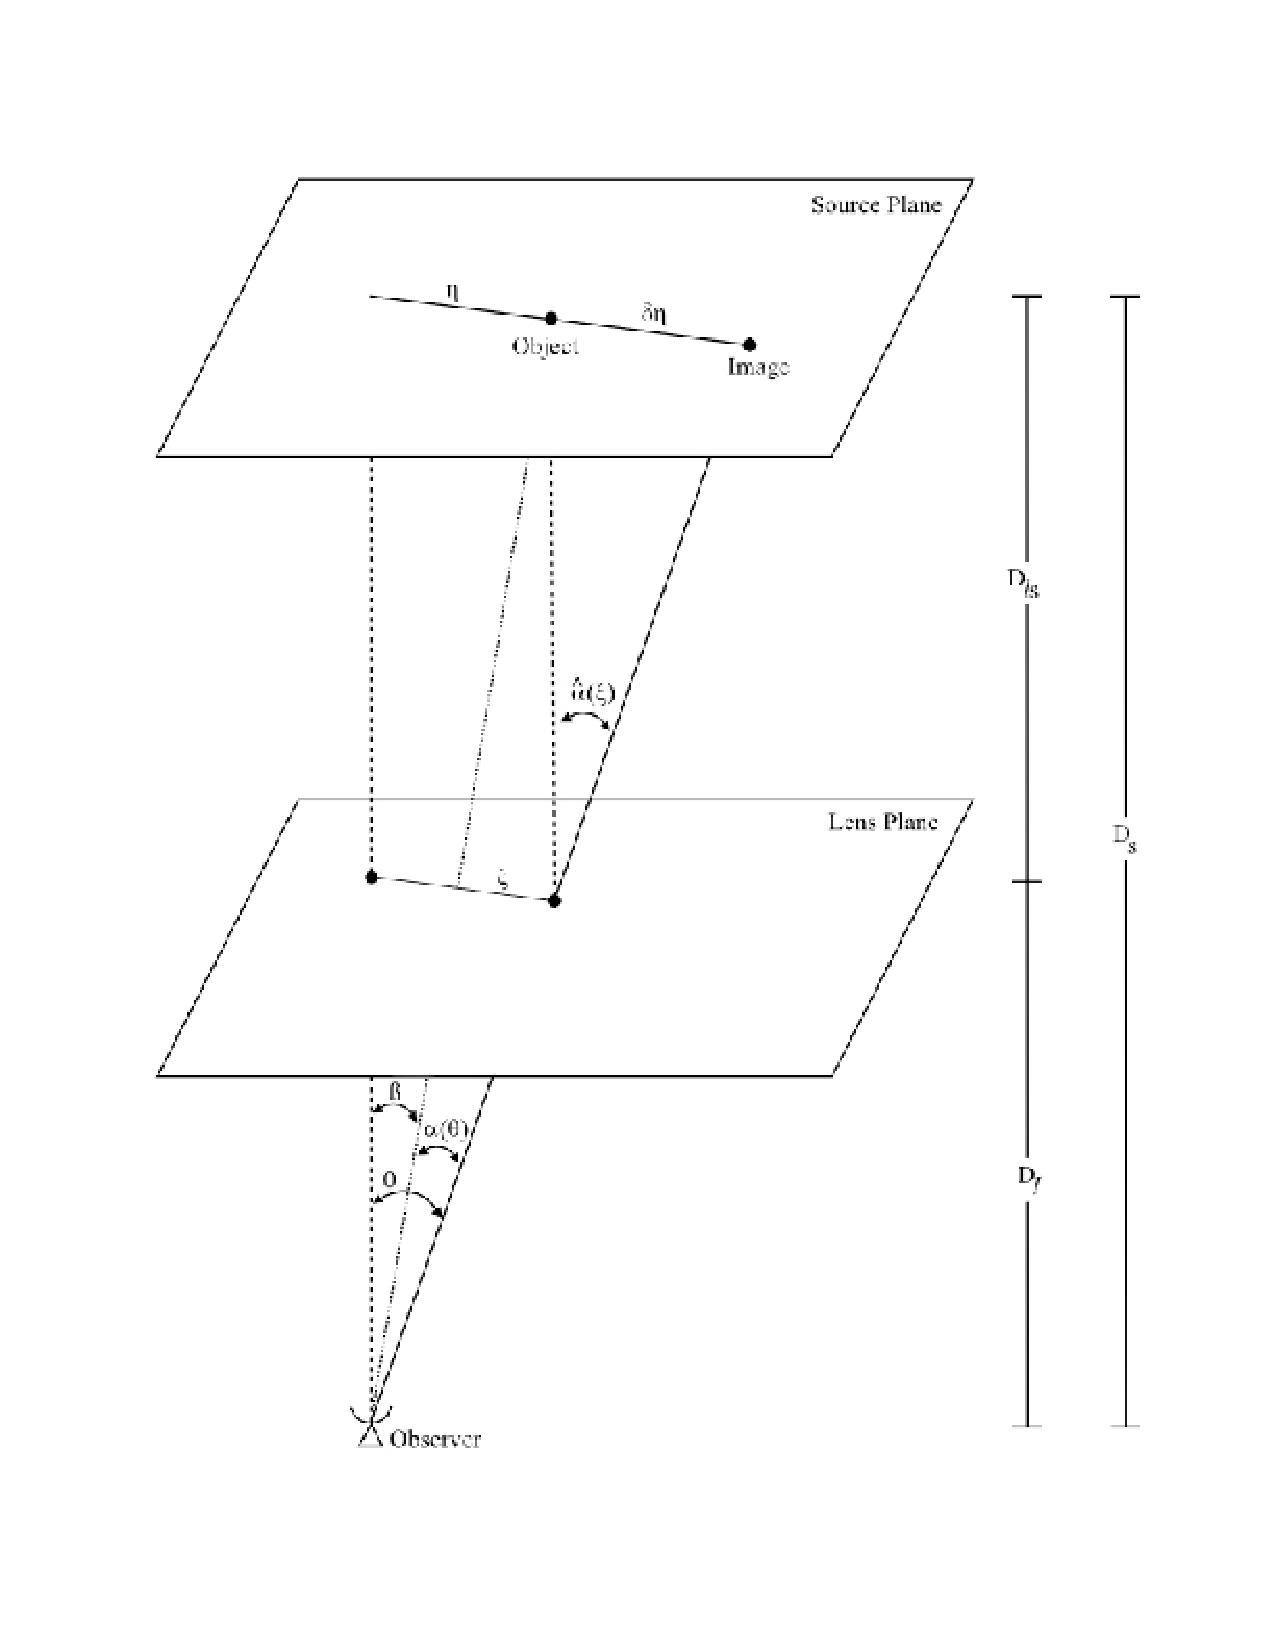
\includegraphics[width=0.5\textwidth]{lensing2}
%   \caption{Simple sketch to gravitational lensing. (Bartelmann and Schneider 2001)} % cite this
% \end{figure}



\newpage
% \bibliographypath{{.bib/}{../bib/}} % comment this and put sections/bib/
\bibliographystyle{plainnat}
\bibliography{prospectus}
\end{document}
